\documentclass[]{article}
\usepackage{lmodern}
\usepackage{amssymb,amsmath}
\usepackage{ifxetex,ifluatex}
\usepackage{fixltx2e} % provides \textsubscript
\ifnum 0\ifxetex 1\fi\ifluatex 1\fi=0 % if pdftex
  \usepackage[T1]{fontenc}
  \usepackage[utf8]{inputenc}
\else % if luatex or xelatex
  \ifxetex
    \usepackage{mathspec}
  \else
    \usepackage{fontspec}
  \fi
  \defaultfontfeatures{Ligatures=TeX,Scale=MatchLowercase}
\fi
% use upquote if available, for straight quotes in verbatim environments
\IfFileExists{upquote.sty}{\usepackage{upquote}}{}
% use microtype if available
\IfFileExists{microtype.sty}{%
\usepackage{microtype}
\UseMicrotypeSet[protrusion]{basicmath} % disable protrusion for tt fonts
}{}
\usepackage[margin=1in]{geometry}
\usepackage{hyperref}
\hypersetup{unicode=true,
            pdftitle={Python in R},
            pdfauthor={Yongbock(David) Kwon},
            pdfborder={0 0 0},
            breaklinks=true}
\urlstyle{same}  % don't use monospace font for urls
\usepackage{color}
\usepackage{fancyvrb}
\newcommand{\VerbBar}{|}
\newcommand{\VERB}{\Verb[commandchars=\\\{\}]}
\DefineVerbatimEnvironment{Highlighting}{Verbatim}{commandchars=\\\{\}}
% Add ',fontsize=\small' for more characters per line
\usepackage{framed}
\definecolor{shadecolor}{RGB}{248,248,248}
\newenvironment{Shaded}{\begin{snugshade}}{\end{snugshade}}
\newcommand{\AlertTok}[1]{\textcolor[rgb]{0.94,0.16,0.16}{#1}}
\newcommand{\AnnotationTok}[1]{\textcolor[rgb]{0.56,0.35,0.01}{\textbf{\textit{#1}}}}
\newcommand{\AttributeTok}[1]{\textcolor[rgb]{0.77,0.63,0.00}{#1}}
\newcommand{\BaseNTok}[1]{\textcolor[rgb]{0.00,0.00,0.81}{#1}}
\newcommand{\BuiltInTok}[1]{#1}
\newcommand{\CharTok}[1]{\textcolor[rgb]{0.31,0.60,0.02}{#1}}
\newcommand{\CommentTok}[1]{\textcolor[rgb]{0.56,0.35,0.01}{\textit{#1}}}
\newcommand{\CommentVarTok}[1]{\textcolor[rgb]{0.56,0.35,0.01}{\textbf{\textit{#1}}}}
\newcommand{\ConstantTok}[1]{\textcolor[rgb]{0.00,0.00,0.00}{#1}}
\newcommand{\ControlFlowTok}[1]{\textcolor[rgb]{0.13,0.29,0.53}{\textbf{#1}}}
\newcommand{\DataTypeTok}[1]{\textcolor[rgb]{0.13,0.29,0.53}{#1}}
\newcommand{\DecValTok}[1]{\textcolor[rgb]{0.00,0.00,0.81}{#1}}
\newcommand{\DocumentationTok}[1]{\textcolor[rgb]{0.56,0.35,0.01}{\textbf{\textit{#1}}}}
\newcommand{\ErrorTok}[1]{\textcolor[rgb]{0.64,0.00,0.00}{\textbf{#1}}}
\newcommand{\ExtensionTok}[1]{#1}
\newcommand{\FloatTok}[1]{\textcolor[rgb]{0.00,0.00,0.81}{#1}}
\newcommand{\FunctionTok}[1]{\textcolor[rgb]{0.00,0.00,0.00}{#1}}
\newcommand{\ImportTok}[1]{#1}
\newcommand{\InformationTok}[1]{\textcolor[rgb]{0.56,0.35,0.01}{\textbf{\textit{#1}}}}
\newcommand{\KeywordTok}[1]{\textcolor[rgb]{0.13,0.29,0.53}{\textbf{#1}}}
\newcommand{\NormalTok}[1]{#1}
\newcommand{\OperatorTok}[1]{\textcolor[rgb]{0.81,0.36,0.00}{\textbf{#1}}}
\newcommand{\OtherTok}[1]{\textcolor[rgb]{0.56,0.35,0.01}{#1}}
\newcommand{\PreprocessorTok}[1]{\textcolor[rgb]{0.56,0.35,0.01}{\textit{#1}}}
\newcommand{\RegionMarkerTok}[1]{#1}
\newcommand{\SpecialCharTok}[1]{\textcolor[rgb]{0.00,0.00,0.00}{#1}}
\newcommand{\SpecialStringTok}[1]{\textcolor[rgb]{0.31,0.60,0.02}{#1}}
\newcommand{\StringTok}[1]{\textcolor[rgb]{0.31,0.60,0.02}{#1}}
\newcommand{\VariableTok}[1]{\textcolor[rgb]{0.00,0.00,0.00}{#1}}
\newcommand{\VerbatimStringTok}[1]{\textcolor[rgb]{0.31,0.60,0.02}{#1}}
\newcommand{\WarningTok}[1]{\textcolor[rgb]{0.56,0.35,0.01}{\textbf{\textit{#1}}}}
\usepackage{graphicx,grffile}
\makeatletter
\def\maxwidth{\ifdim\Gin@nat@width>\linewidth\linewidth\else\Gin@nat@width\fi}
\def\maxheight{\ifdim\Gin@nat@height>\textheight\textheight\else\Gin@nat@height\fi}
\makeatother
% Scale images if necessary, so that they will not overflow the page
% margins by default, and it is still possible to overwrite the defaults
% using explicit options in \includegraphics[width, height, ...]{}
\setkeys{Gin}{width=\maxwidth,height=\maxheight,keepaspectratio}
\IfFileExists{parskip.sty}{%
\usepackage{parskip}
}{% else
\setlength{\parindent}{0pt}
\setlength{\parskip}{6pt plus 2pt minus 1pt}
}
\setlength{\emergencystretch}{3em}  % prevent overfull lines
\providecommand{\tightlist}{%
  \setlength{\itemsep}{0pt}\setlength{\parskip}{0pt}}
\setcounter{secnumdepth}{0}
% Redefines (sub)paragraphs to behave more like sections
\ifx\paragraph\undefined\else
\let\oldparagraph\paragraph
\renewcommand{\paragraph}[1]{\oldparagraph{#1}\mbox{}}
\fi
\ifx\subparagraph\undefined\else
\let\oldsubparagraph\subparagraph
\renewcommand{\subparagraph}[1]{\oldsubparagraph{#1}\mbox{}}
\fi

%%% Use protect on footnotes to avoid problems with footnotes in titles
\let\rmarkdownfootnote\footnote%
\def\footnote{\protect\rmarkdownfootnote}

%%% Change title format to be more compact
\usepackage{titling}

% Create subtitle command for use in maketitle
\providecommand{\subtitle}[1]{
  \posttitle{
    \begin{center}\large#1\end{center}
    }
}

\setlength{\droptitle}{-2em}

  \title{Python in R}
    \pretitle{\vspace{\droptitle}\centering\huge}
  \posttitle{\par}
    \author{Yongbock(David) Kwon}
    \preauthor{\centering\large\emph}
  \postauthor{\par}
    \date{}
    \predate{}\postdate{}
  

\begin{document}
\maketitle

\begin{Shaded}
\begin{Highlighting}[]
\KeywordTok{library}\NormalTok{(caret)}
\end{Highlighting}
\end{Shaded}

\begin{verbatim}
## Loading required package: lattice
\end{verbatim}

\begin{verbatim}
## Loading required package: ggplot2
\end{verbatim}

\begin{verbatim}
## Registered S3 methods overwritten by 'ggplot2':
##   method         from 
##   [.quosures     rlang
##   c.quosures     rlang
##   print.quosures rlang
\end{verbatim}

\begin{Shaded}
\begin{Highlighting}[]
\KeywordTok{library}\NormalTok{(rpart)}
\KeywordTok{library}\NormalTok{(rpart.plot)}
\KeywordTok{library}\NormalTok{(ggplot2)}
\KeywordTok{library}\NormalTok{(dplyr)}
\end{Highlighting}
\end{Shaded}

\begin{verbatim}
## 
## Attaching package: 'dplyr'
\end{verbatim}

\begin{verbatim}
## The following objects are masked from 'package:stats':
## 
##     filter, lag
\end{verbatim}

\begin{verbatim}
## The following objects are masked from 'package:base':
## 
##     intersect, setdiff, setequal, union
\end{verbatim}

\begin{Shaded}
\begin{Highlighting}[]
\KeywordTok{library}\NormalTok{(gridExtra)}
\end{Highlighting}
\end{Shaded}

\begin{verbatim}
## 
## Attaching package: 'gridExtra'
\end{verbatim}

\begin{verbatim}
## The following object is masked from 'package:dplyr':
## 
##     combine
\end{verbatim}

\begin{Shaded}
\begin{Highlighting}[]
\CommentTok{#Quick Decision Tree in R}
\NormalTok{iris1 <-}\StringTok{ }\NormalTok{iris[}\KeywordTok{which}\NormalTok{(iris}\OperatorTok{$}\NormalTok{Species }\OperatorTok{!=}\StringTok{ "virginica"}\NormalTok{),]}

\CommentTok{#removing the factor level that we don't have any more}
\NormalTok{iris1}\OperatorTok{$}\NormalTok{Species <-}\StringTok{ }\KeywordTok{as.factor}\NormalTok{(}\KeywordTok{as.character}\NormalTok{(iris1}\OperatorTok{$}\NormalTok{Species))}

\KeywordTok{set.seed}\NormalTok{(}\DecValTok{1234}\NormalTok{)}
\CommentTok{#splitting dataset}
\NormalTok{training.idx <-}\StringTok{ }\KeywordTok{createDataPartition}\NormalTok{(iris1}\OperatorTok{$}\NormalTok{Species, }\DataTypeTok{p=}\FloatTok{0.7}\NormalTok{, }\DataTypeTok{list=}\OtherTok{FALSE}\NormalTok{)}

\NormalTok{training <-}\StringTok{ }\NormalTok{iris1[training.idx,]}
\NormalTok{testing <-}\StringTok{ }\NormalTok{iris1[}\OperatorTok{-}\NormalTok{training.idx,]}

\CommentTok{#quick decision tree built in r, rpart}
\NormalTok{tr <-}\StringTok{ }\KeywordTok{rpart}\NormalTok{(Species}\OperatorTok{~}\NormalTok{., training)}
\NormalTok{tr}
\end{Highlighting}
\end{Shaded}

\begin{verbatim}
## n= 70 
## 
## node), split, n, loss, yval, (yprob)
##       * denotes terminal node
## 
## 1) root 70 35 setosa (0.5000000 0.5000000)  
##   2) Petal.Length< 2.35 35  0 setosa (1.0000000 0.0000000) *
##   3) Petal.Length>=2.35 35  0 versicolor (0.0000000 1.0000000) *
\end{verbatim}

\begin{Shaded}
\begin{Highlighting}[]
\KeywordTok{rpart.plot}\NormalTok{(tr)}
\end{Highlighting}
\end{Shaded}

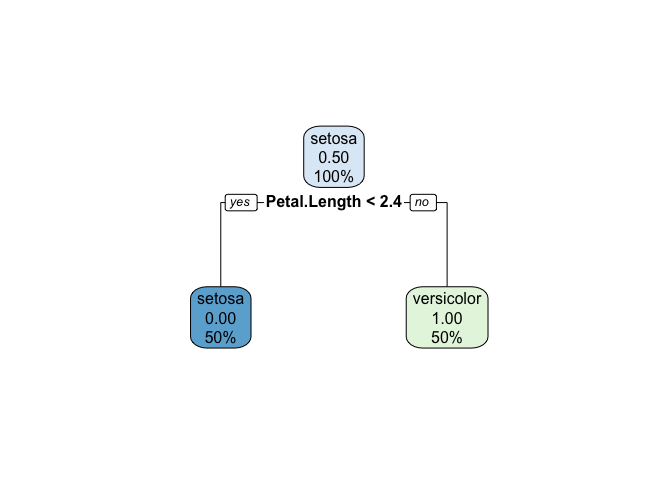
\includegraphics{PythonInR_files/figure-latex/inR-1.pdf}

\begin{Shaded}
\begin{Highlighting}[]
\NormalTok{dtree.pred <-}\StringTok{ }\KeywordTok{predict}\NormalTok{(tr, }\DataTypeTok{type=}\StringTok{"class"}\NormalTok{)}

\KeywordTok{table}\NormalTok{(dtree.pred, training}\OperatorTok{$}\NormalTok{Species)}
\end{Highlighting}
\end{Shaded}

\begin{verbatim}
##             
## dtree.pred   setosa versicolor
##   setosa         35          0
##   versicolor      0         35
\end{verbatim}

\begin{Shaded}
\begin{Highlighting}[]
\CommentTok{#with Petal.Length < 2.5, the model predict perfectly in training set}

\NormalTok{dtree.pred.test <-}\StringTok{ }\KeywordTok{predict}\NormalTok{(tr, testing, }\DataTypeTok{type=}\StringTok{"class"}\NormalTok{)}

\KeywordTok{table}\NormalTok{(dtree.pred.test, testing}\OperatorTok{$}\NormalTok{Species)}
\end{Highlighting}
\end{Shaded}

\begin{verbatim}
##                
## dtree.pred.test setosa versicolor
##      setosa         15          0
##      versicolor      0         15
\end{verbatim}

\begin{Shaded}
\begin{Highlighting}[]
\CommentTok{#with Petal.Length < 2.5, the model predict perfectly in testing set as well}


\NormalTok{t1 <-}\StringTok{ }\NormalTok{testing }\OperatorTok\StringTok{ }
\StringTok{  }\KeywordTok{ggplot}\NormalTok{(}\KeywordTok{aes}\NormalTok{(}\DataTypeTok{x=}\NormalTok{Petal.Length, }\DataTypeTok{y=}\NormalTok{Petal.Width, }\DataTypeTok{col=}\NormalTok{Species)) }\OperatorTok{+}\StringTok{ }
\StringTok{  }\KeywordTok{geom_jitter}\NormalTok{() }\OperatorTok{+}\StringTok{ }\KeywordTok{ggtitle}\NormalTok{(}\StringTok{"Actual value in R"}\NormalTok{)}
\NormalTok{t2 <-}\StringTok{ }\NormalTok{testing }\OperatorTok\StringTok{ }
\StringTok{  }\KeywordTok{ggplot}\NormalTok{(}\KeywordTok{aes}\NormalTok{(}\DataTypeTok{x=}\NormalTok{Petal.Length, }\DataTypeTok{y=}\NormalTok{Petal.Width, }\DataTypeTok{col=}\NormalTok{dtree.pred.test)) }\OperatorTok{+}\StringTok{ }
\StringTok{  }\KeywordTok{geom_jitter}\NormalTok{() }\OperatorTok{+}\StringTok{ }\KeywordTok{ggtitle}\NormalTok{(}\StringTok{"Predicted value in R"}\NormalTok{)}
\KeywordTok{grid.arrange}\NormalTok{(t1, t2) }
\end{Highlighting}
\end{Shaded}

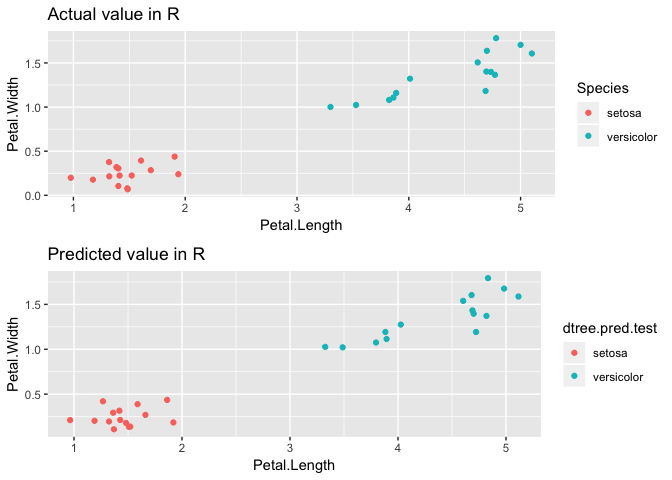
\includegraphics{PythonInR_files/figure-latex/inR-2.pdf}

\begin{Shaded}
\begin{Highlighting}[]
\KeywordTok{library}\NormalTok{(reticulate)}
\CommentTok{#Let's use conda environment}
\KeywordTok{Sys.which}\NormalTok{(}\StringTok{"python"}\NormalTok{)}
\end{Highlighting}
\end{Shaded}

\begin{verbatim}
##            python 
## "/usr/bin/python"
\end{verbatim}

\begin{Shaded}
\begin{Highlighting}[]
\KeywordTok{use_python}\NormalTok{(}\StringTok{"/anaconda3/bin/python"}\NormalTok{)}

\KeywordTok{virtualenv_list}\NormalTok{()}
\end{Highlighting}
\end{Shaded}

\begin{verbatim}
## [1] "r-reticulate"
\end{verbatim}

\begin{Shaded}
\begin{Highlighting}[]
\CommentTok{#you have to reopen Rstudio after installing those packages into virtual environment}
\CommentTok{#also make sure you have installed the packages in conda environment}

\CommentTok{#virtualenv_install("r-reticulate", "bayesian-optimization")}
\CommentTok{#virtualenv_install("r-reticulate", "pandas")}
\CommentTok{#virtualenv_install("r-reticulate", "seaborn")}
\CommentTok{#virtualenv_install("r-reticulate", "sklearn")}
\CommentTok{#virtualenv_install("r-reticulate", "xgboost")}
\KeywordTok{use_virtualenv}\NormalTok{(}\StringTok{"r-reticulate"}\NormalTok{)}



\KeywordTok{py_module_available}\NormalTok{(}\StringTok{"seaborn"}\NormalTok{)}
\end{Highlighting}
\end{Shaded}

\begin{verbatim}
## [1] TRUE
\end{verbatim}

\begin{Shaded}
\begin{Highlighting}[]
\KeywordTok{py_module_available}\NormalTok{(}\StringTok{"sklearn"}\NormalTok{)}
\end{Highlighting}
\end{Shaded}

\begin{verbatim}
## [1] TRUE
\end{verbatim}

\begin{Shaded}
\begin{Highlighting}[]
\KeywordTok{py_module_available}\NormalTok{(}\StringTok{"pandas"}\NormalTok{)}
\end{Highlighting}
\end{Shaded}

\begin{verbatim}
## [1] TRUE
\end{verbatim}

\begin{Shaded}
\begin{Highlighting}[]
\KeywordTok{py_module_available}\NormalTok{(}\StringTok{"bayes_opt"}\NormalTok{)}
\end{Highlighting}
\end{Shaded}

\begin{verbatim}
## [1] TRUE
\end{verbatim}

\begin{Shaded}
\begin{Highlighting}[]
\KeywordTok{py_module_available}\NormalTok{(}\StringTok{"xgboost"}\NormalTok{)}
\end{Highlighting}
\end{Shaded}

\begin{verbatim}
## [1] TRUE
\end{verbatim}

Install pip with: \$ /usr/bin/python -m easy\_install --upgrade --user
pip

Install virtualenv with: \$ /usr/bin/python -m pip install --upgrade
--user virtualenv

\begin{Shaded}
\begin{Highlighting}[]

\ImportTok{import}\NormalTok{ matplotlib }\ImportTok{as}\NormalTok{ mlt}
\ImportTok{import}\NormalTok{ matplotlib.pyplot }\ImportTok{as}\NormalTok{ plt}
\ImportTok{import}\NormalTok{ numpy }\ImportTok{as}\NormalTok{ np}
\ImportTok{import}\NormalTok{ seaborn }\ImportTok{as}\NormalTok{ sns}
\ImportTok{import}\NormalTok{ pandas }\ImportTok{as}\NormalTok{ pd}
\ImportTok{from}\NormalTok{ sklearn.datasets }\ImportTok{import}\NormalTok{ load_iris}
\ImportTok{from}\NormalTok{ sklearn }\ImportTok{import}\NormalTok{ tree}
\ImportTok{from}\NormalTok{ sklearn.model_selection }\ImportTok{import}\NormalTok{ cross_val_score}
\ImportTok{from}\NormalTok{ sklearn.model_selection }\ImportTok{import}\NormalTok{ train_test_split}
\CommentTok{#iris dataset that I have removed the row for virginica in Species}
\NormalTok{r.iris1.head(}\DecValTok{5}\NormalTok{)}
\end{Highlighting}
\end{Shaded}

\begin{verbatim}
##    Sepal.Length  Sepal.Width  Petal.Length  Petal.Width Species
## 0           5.1          3.5           1.4          0.2  setosa
## 1           4.9          3.0           1.4          0.2  setosa
## 2           4.7          3.2           1.3          0.2  setosa
## 3           4.6          3.1           1.5          0.2  setosa
## 4           5.0          3.6           1.4          0.2  setosa
\end{verbatim}

\begin{Shaded}
\begin{Highlighting}[]
\NormalTok{r.iris1.describe()}

\CommentTok{#Let's create same datset from iris in Python module, it's in "new" virtual environment}
\CommentTok{#import iris dataset from sklearn}
\end{Highlighting}
\end{Shaded}

\begin{verbatim}
##        Sepal.Length  Sepal.Width  Petal.Length  Petal.Width
## count    100.000000   100.000000    100.000000   100.000000
## mean       5.471000     3.099000      2.861000     0.786000
## std        0.641698     0.478739      1.449549     0.565153
## min        4.300000     2.000000      1.000000     0.100000
## 25%        5.000000     2.800000      1.500000     0.200000
## 50%        5.400000     3.050000      2.450000     0.800000
## 75%        5.900000     3.400000      4.325000     1.300000
## max        7.000000     4.400000      5.100000     1.800000
\end{verbatim}

\begin{Shaded}
\begin{Highlighting}[]
\NormalTok{iris2 }\OperatorTok{=}\NormalTok{ load_iris()}

\NormalTok{r.iris1.columns}

\CommentTok{#convert sklearn dataset to pandas dataframe}
\end{Highlighting}
\end{Shaded}

\begin{verbatim}
## Index(['Sepal.Length', 'Sepal.Width', 'Petal.Length', 'Petal.Width',
##        'Species'],
##       dtype='object')
\end{verbatim}

\begin{Shaded}
\begin{Highlighting}[]
\NormalTok{df_iris2 }\OperatorTok{=}\NormalTok{ pd.DataFrame(data}\OperatorTok{=}\NormalTok{ np.c_[iris2[}\StringTok{'data'}\NormalTok{], iris2[}\StringTok{'target'}\NormalTok{]], columns}\OperatorTok{=}\NormalTok{ [}\StringTok{'SepalLength'}\NormalTok{,}\StringTok{'SepalWidth'}\NormalTok{,}\StringTok{'PetalLength'}\NormalTok{,}\StringTok{'PetalWidth'}\NormalTok{,}\StringTok{'Species'}\NormalTok{])}

\NormalTok{df_iris2.head(}\DecValTok{5}\NormalTok{)}

\CommentTok{#remove "virginica" }
\end{Highlighting}
\end{Shaded}

\begin{verbatim}
##    SepalLength  SepalWidth  PetalLength  PetalWidth  Species
## 0          5.1         3.5          1.4         0.2      0.0
## 1          4.9         3.0          1.4         0.2      0.0
## 2          4.7         3.2          1.3         0.2      0.0
## 3          4.6         3.1          1.5         0.2      0.0
## 4          5.0         3.6          1.4         0.2      0.0
\end{verbatim}

\begin{Shaded}
\begin{Highlighting}[]
\NormalTok{new_iris2 }\OperatorTok{=}\NormalTok{ df_iris2[df_iris2.Species }\OperatorTok{!=}\DecValTok{2}\NormalTok{]}

\NormalTok{Y }\OperatorTok{=}\NormalTok{ new_iris2.Species}
\NormalTok{X }\OperatorTok{=}\NormalTok{ new_iris2.iloc[:,}\DecValTok{0}\NormalTok{:}\DecValTok{4}\NormalTok{]}

\NormalTok{X_train, X_test, y_train, y_test }\OperatorTok{=}\NormalTok{ train_test_split(X, Y, test_size}\OperatorTok{=}\FloatTok{0.3}\NormalTok{, random_state}\OperatorTok{=}\DecValTok{42}\NormalTok{)}

\NormalTok{tree_clf }\OperatorTok{=}\NormalTok{ tree.DecisionTreeClassifier(max_depth}\OperatorTok{=}\DecValTok{2}\NormalTok{, random_state}\OperatorTok{=}\DecValTok{42}\NormalTok{)}
\NormalTok{cross_val_score(tree_clf, X_train, y_train, cv}\OperatorTok{=}\DecValTok{10}\NormalTok{)}
\end{Highlighting}
\end{Shaded}

\begin{verbatim}
## array([1., 1., 1., 1., 1., 1., 1., 1., 1., 1.])
\end{verbatim}

\begin{Shaded}
\begin{Highlighting}[]
\NormalTok{tree_fit }\OperatorTok{=}\NormalTok{ tree_clf.fit(X_train, y_train)}
\NormalTok{tree_fit}
\end{Highlighting}
\end{Shaded}

\begin{verbatim}
## DecisionTreeClassifier(class_weight=None, criterion='gini', max_depth=2,
##             max_features=None, max_leaf_nodes=None,
##             min_impurity_decrease=0.0, min_impurity_split=None,
##             min_samples_leaf=1, min_samples_split=2,
##             min_weight_fraction_leaf=0.0, presort=False, random_state=42,
##             splitter='best')
\end{verbatim}

\begin{Shaded}
\begin{Highlighting}[]
\NormalTok{pred }\OperatorTok{=}\NormalTok{ tree_clf.predict(X_test)}

\NormalTok{pd.crosstab(pred, y_test, rownames }\OperatorTok{=}\NormalTok{ [}\StringTok{'pred'}\NormalTok{], colnames}\OperatorTok{=}\NormalTok{[}\StringTok{'actual'}\NormalTok{])}
\end{Highlighting}
\end{Shaded}

\begin{verbatim}
## actual  0.0  1.0
## pred            
## 0.0      17    0
## 1.0       0   13
\end{verbatim}

\begin{Shaded}
\begin{Highlighting}[]
\NormalTok{plt.subplot(}\DecValTok{1}\NormalTok{, }\DecValTok{2}\NormalTok{, }\DecValTok{1}\NormalTok{)}
\NormalTok{plt.scatter(X_test.PetalLength, X_test.PetalWidth, c}\OperatorTok{=}\NormalTok{pred)}
\NormalTok{plt.title(}\StringTok{'Predicted value'}\NormalTok{)}
\NormalTok{plt.subplot(}\DecValTok{1}\NormalTok{, }\DecValTok{2}\NormalTok{, }\DecValTok{2}\NormalTok{)}
\NormalTok{plt.scatter(X_test.PetalLength, X_test.PetalWidth, c}\OperatorTok{=}\NormalTok{y_test)}
\NormalTok{plt.title(}\StringTok{'Actual value'}\NormalTok{)}
\NormalTok{plt.show()}
\end{Highlighting}
\end{Shaded}

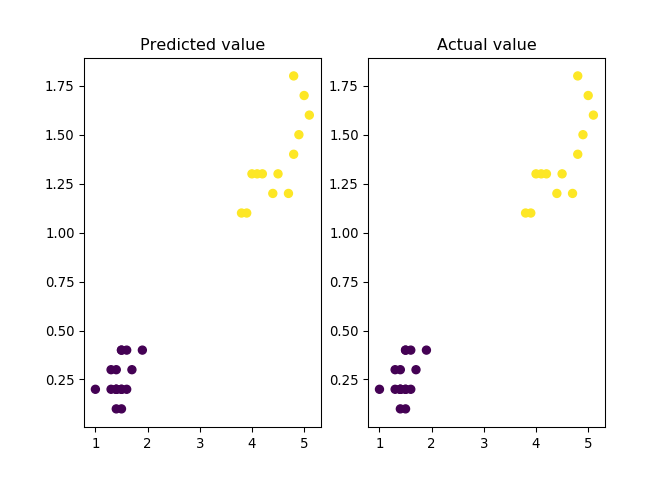
\includegraphics{PythonInR_files/figure-latex/inPython-1.pdf}

\begin{Shaded}
\begin{Highlighting}[]
\CommentTok{#see the created Dataset from Python}
\KeywordTok{library}\NormalTok{(plyr)}
\end{Highlighting}
\end{Shaded}

\begin{verbatim}
## -------------------------------------------------------------------------
\end{verbatim}

\begin{verbatim}
## You have loaded plyr after dplyr - this is likely to cause problems.
## If you need functions from both plyr and dplyr, please load plyr first, then dplyr:
## library(plyr); library(dplyr)
\end{verbatim}

\begin{verbatim}
## -------------------------------------------------------------------------
\end{verbatim}

\begin{verbatim}
## 
## Attaching package: 'plyr'
\end{verbatim}

\begin{verbatim}
## The following objects are masked from 'package:dplyr':
## 
##     arrange, count, desc, failwith, id, mutate, rename, summarise,
##     summarize
\end{verbatim}

\begin{Shaded}
\begin{Highlighting}[]
\NormalTok{iris.convert <-}\StringTok{ }\ControlFlowTok{function}\NormalTok{(Y)\{}
\NormalTok{  y <-}\StringTok{ }\KeywordTok{as.character}\NormalTok{(Y)}
\NormalTok{  y <-}\StringTok{ }\KeywordTok{as.factor}\NormalTok{(}\KeywordTok{revalue}\NormalTok{(y,}\KeywordTok{c}\NormalTok{(}\StringTok{'0'}\NormalTok{ =}\StringTok{ "setosa"}\NormalTok{, }\StringTok{'1'}\NormalTok{ =}\StringTok{ "versicolor"}\NormalTok{)))}
  \KeywordTok{return}\NormalTok{(y)}
\NormalTok{\}}

\NormalTok{py.act <-}\StringTok{ }\NormalTok{py}\OperatorTok{$}\NormalTok{X_test }\OperatorTok\StringTok{ }
\StringTok{  }\KeywordTok{mutate}\NormalTok{(}\DataTypeTok{act =} \KeywordTok{iris.convert}\NormalTok{(py}\OperatorTok{$}\NormalTok{y_test)) }\OperatorTok\StringTok{ }
\StringTok{  }\KeywordTok{ggplot}\NormalTok{(}\KeywordTok{aes}\NormalTok{(}\DataTypeTok{x=}\NormalTok{PetalLength, }\DataTypeTok{y=}\NormalTok{PetalWidth, }\DataTypeTok{col=}\NormalTok{act)) }\OperatorTok{+}\StringTok{ }
\StringTok{  }\KeywordTok{geom_jitter}\NormalTok{()}\OperatorTok{+}
\StringTok{  }\KeywordTok{labs}\NormalTok{(}\DataTypeTok{title=}\StringTok{"Actual Value in Python"}\NormalTok{)}

\NormalTok{py.pred <-}\StringTok{ }\NormalTok{py}\OperatorTok{$}\NormalTok{X_test }\OperatorTok\StringTok{ }
\StringTok{  }\KeywordTok{mutate}\NormalTok{(}\DataTypeTok{pred =} \KeywordTok{iris.convert}\NormalTok{(py}\OperatorTok{$}\NormalTok{pred)) }\OperatorTok\StringTok{ }
\StringTok{  }\KeywordTok{ggplot}\NormalTok{(}\KeywordTok{aes}\NormalTok{(}\DataTypeTok{x=}\NormalTok{PetalLength, }\DataTypeTok{y=}\NormalTok{PetalWidth, }\DataTypeTok{col=}\NormalTok{pred)) }\OperatorTok{+}
\StringTok{  }\KeywordTok{geom_jitter}\NormalTok{()}\OperatorTok{+}
\StringTok{  }\KeywordTok{labs}\NormalTok{(}\DataTypeTok{title=}\StringTok{"Predicted value in Python"}\NormalTok{)}

\KeywordTok{grid.arrange}\NormalTok{(py.act, py.pred) }
\end{Highlighting}
\end{Shaded}

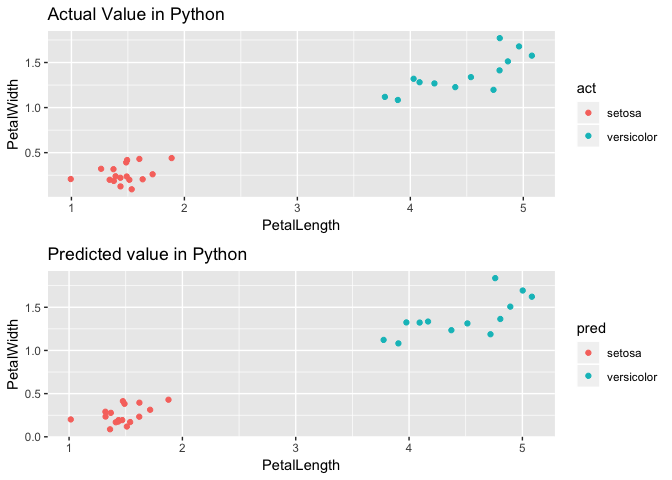
\includegraphics{PythonInR_files/figure-latex/fromPythontoR-1.pdf}

\begin{Shaded}
\begin{Highlighting}[]
\KeywordTok{grid.arrange}\NormalTok{(t1,t2)}
\end{Highlighting}
\end{Shaded}

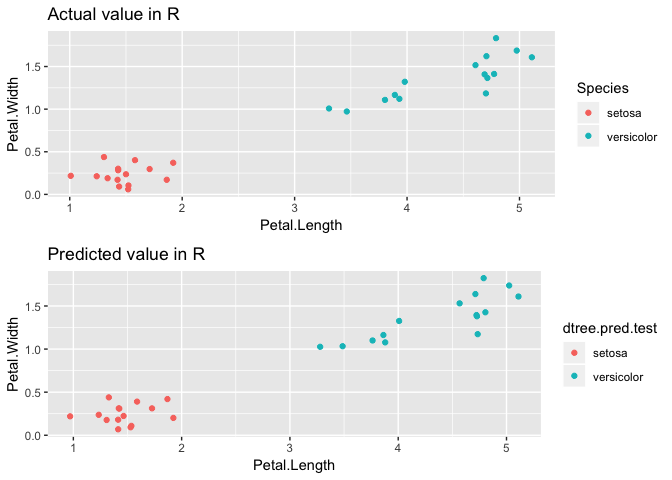
\includegraphics{PythonInR_files/figure-latex/fromPythontoR-2.pdf}

\begin{Shaded}
\begin{Highlighting}[]
\KeywordTok{detach}\NormalTok{(package}\OperatorTok{:}\NormalTok{plyr)}
\end{Highlighting}
\end{Shaded}

\begin{Shaded}
\begin{Highlighting}[]
\KeywordTok{library}\NormalTok{(xgboost)}
\end{Highlighting}
\end{Shaded}

\begin{verbatim}
## 
## Attaching package: 'xgboost'
\end{verbatim}

\begin{verbatim}
## The following object is masked from 'package:dplyr':
## 
##     slice
\end{verbatim}

\begin{Shaded}
\begin{Highlighting}[]
\KeywordTok{library}\NormalTok{(rBayesianOptimization)}
\KeywordTok{library}\NormalTok{(MLmetrics)}
\end{Highlighting}
\end{Shaded}

\begin{verbatim}
## 
## Attaching package: 'MLmetrics'
\end{verbatim}

\begin{verbatim}
## The following objects are masked from 'package:caret':
## 
##     MAE, RMSE
\end{verbatim}

\begin{verbatim}
## The following object is masked from 'package:base':
## 
##     Recall
\end{verbatim}

\begin{Shaded}
\begin{Highlighting}[]
\CommentTok{#Let's remove all environment created above}
\KeywordTok{rm}\NormalTok{(}\DataTypeTok{list=}\KeywordTok{ls}\NormalTok{())}

\CommentTok{#labeling species}
\NormalTok{iris1 <-}\StringTok{ }\NormalTok{iris }\OperatorTok\StringTok{ }\KeywordTok{mutate}\NormalTok{(}\DataTypeTok{Species =} \KeywordTok{as.integer}\NormalTok{(Species)}\OperatorTok{-}\DecValTok{1}\NormalTok{)}

\KeywordTok{set.seed}\NormalTok{(}\DecValTok{1234}\NormalTok{)}
\CommentTok{#splitting dataset}
\NormalTok{training.idx <-}\StringTok{ }\KeywordTok{createDataPartition}\NormalTok{(iris1}\OperatorTok{$}\NormalTok{Species, }\DataTypeTok{p=}\FloatTok{0.7}\NormalTok{, }\DataTypeTok{list=}\OtherTok{FALSE}\NormalTok{)}

\CommentTok{#splitting}
\NormalTok{train <-}\StringTok{ }\KeywordTok{as.matrix}\NormalTok{(iris1[training.idx,])}
\NormalTok{valid <-}\StringTok{ }\KeywordTok{as.matrix}\NormalTok{(iris1[}\OperatorTok{-}\NormalTok{training.idx,])}

\NormalTok{train.label <-}\StringTok{ }\NormalTok{iris1}\OperatorTok{$}\NormalTok{Species[training.idx]}
\NormalTok{valid.label <-}\StringTok{ }\NormalTok{iris1}\OperatorTok{$}\NormalTok{Species[}\OperatorTok{-}\NormalTok{training.idx]}

\CommentTok{#XGB dataform}
\NormalTok{dtrain <-}\StringTok{ }\KeywordTok{xgb.DMatrix}\NormalTok{(}\DataTypeTok{data =} \KeywordTok{as.matrix}\NormalTok{(train),}
                      \DataTypeTok{label =}\NormalTok{ train.label)}
\NormalTok{dvalid <-}\StringTok{ }\KeywordTok{xgb.DMatrix}\NormalTok{(}\DataTypeTok{data =} \KeywordTok{as.matrix}\NormalTok{(valid),}
                      \DataTypeTok{label =}\NormalTok{ valid.label)}

\KeywordTok{set.seed}\NormalTok{(}\DecValTok{1234}\NormalTok{)}
\CommentTok{#cv}
\NormalTok{cv_folds <-}\StringTok{ }\KeywordTok{createFolds}\NormalTok{(train.label, }\DataTypeTok{k=}\DecValTok{5}\NormalTok{, }\DataTypeTok{list=}\OtherTok{TRUE}\NormalTok{)}

\CommentTok{#function for bayesian optimization}
\NormalTok{xgb_cv_bayes <-}\StringTok{ }\ControlFlowTok{function}\NormalTok{(max_depth, min_child_weight, subsample, }
\NormalTok{                         colsample_bytree, lambda, gamma, alpha) \{}
\NormalTok{  cv <-}\StringTok{ }\KeywordTok{xgb.cv}\NormalTok{(}\DataTypeTok{params =} \KeywordTok{list}\NormalTok{(}\DataTypeTok{booster =} \StringTok{"gbtree"}\NormalTok{, }\DataTypeTok{eta =} \FloatTok{0.008}\NormalTok{,}
                             \DataTypeTok{max_depth =}\NormalTok{ max_depth,}
                             \DataTypeTok{min_child_weight =}\NormalTok{ min_child_weight,}
                             \DataTypeTok{subsample =}\NormalTok{ subsample, }
                             \DataTypeTok{colsample_bytree =}\NormalTok{ colsample_bytree,}
                             \DataTypeTok{lambda =}\NormalTok{ lambda, }
                             \DataTypeTok{gamma =}\NormalTok{ gamma,}
                             \DataTypeTok{alpha =}\NormalTok{ alpha,}
                             \DataTypeTok{objective =} \StringTok{"multi:softprob"}\NormalTok{,}
                             \DataTypeTok{eval_metric =} \StringTok{"mlogloss"}\NormalTok{,}
                             \DataTypeTok{num_class=}\DecValTok{3}\NormalTok{),}
               \DataTypeTok{data =}\NormalTok{ dtrain, }\DataTypeTok{nround =} \DecValTok{1000}\NormalTok{,}
               \DataTypeTok{folds =}\NormalTok{ cv_folds, }\DataTypeTok{prediction =} \OtherTok{TRUE}\NormalTok{, }\DataTypeTok{showsd =} \OtherTok{TRUE}\NormalTok{,}
               \DataTypeTok{early_stopping_rounds =} \DecValTok{100}\NormalTok{, }\DataTypeTok{maximize =} \OtherTok{TRUE}\NormalTok{, }\DataTypeTok{verbose =} \DecValTok{0}\NormalTok{)}
  \KeywordTok{list}\NormalTok{(}\DataTypeTok{Score =}\NormalTok{ cv}\OperatorTok{$}\NormalTok{evaluation_log}\OperatorTok{$}\NormalTok{test_mlogloss_mean[cv}\OperatorTok{$}\NormalTok{best_iteration],}
       \DataTypeTok{Pred =}\NormalTok{ cv}\OperatorTok{$}\NormalTok{pred)}
\NormalTok{\}}

\CommentTok{#BayesianOptimization}
\NormalTok{Bayes_opt <-}\StringTok{ }\KeywordTok{BayesianOptimization}\NormalTok{(xgb_cv_bayes,}
                                \DataTypeTok{bounds =} \KeywordTok{list}\NormalTok{(}
                                  \CommentTok{#tree depth}
                                  \DataTypeTok{max_depth =} \KeywordTok{c}\NormalTok{(1L,5L), }
                                  \CommentTok{#sum of Hessian for each node}
                                  \DataTypeTok{min_child_weight =} \KeywordTok{c}\NormalTok{(1L, 10L),}
                                  \CommentTok{#randomly sapmle row index(data points)}
                                  \DataTypeTok{subsample =} \KeywordTok{c}\NormalTok{(}\FloatTok{0.6}\NormalTok{, }\DecValTok{1}\NormalTok{),}
                                  \CommentTok{#randomly sample column index(like random forest)}
                                  \DataTypeTok{colsample_bytree =} \KeywordTok{c}\NormalTok{(}\FloatTok{0.6}\NormalTok{,}\DecValTok{1}\NormalTok{),}
                                  \CommentTok{#adding L2 regularization term (ridge)}
                                  \DataTypeTok{lambda =} \KeywordTok{c}\NormalTok{(}\FloatTok{0.001}\NormalTok{,}\DecValTok{1}\NormalTok{),}
                                  \CommentTok{#adding L1 regularization term (lasso)}
                                  \DataTypeTok{alpha =} \KeywordTok{c}\NormalTok{(}\FloatTok{0.001}\NormalTok{,}\DecValTok{1}\NormalTok{),}
                                  \DataTypeTok{gamma =} \KeywordTok{c}\NormalTok{(}\FloatTok{0.1}\NormalTok{,}\DecValTok{2}\NormalTok{)),}
                                \DataTypeTok{init_grid_dt =} \OtherTok{NULL}\NormalTok{, }\DataTypeTok{init_points =} \DecValTok{10}\NormalTok{, }\DataTypeTok{n_iter =} \DecValTok{20}\NormalTok{,}
                                \DataTypeTok{acq =} \StringTok{"ucb"}\NormalTok{, }\DataTypeTok{kappa =} \FloatTok{2.576}\NormalTok{, }\DataTypeTok{eps =} \FloatTok{0.0}\NormalTok{,}
                                \DataTypeTok{verbose =} \OtherTok{TRUE}\NormalTok{)}
\end{Highlighting}
\end{Shaded}

\begin{verbatim}
## elapsed = 0.25   Round = 1   max_depth = 3.0000  min_child_weight = 6.0000   subsample = 0.7301  colsample_bytree = 0.7212   lambda = 0.7428 alpha = 0.6396  gamma = 1.9727  Value = 1.0887 
## elapsed = 0.17   Round = 2   max_depth = 3.0000  min_child_weight = 5.0000   subsample = 0.9029  colsample_bytree = 0.7915   lambda = 0.6393 alpha = 0.6611  gamma = 1.1760  Value = 1.0887 
## elapsed = 0.20   Round = 3   max_depth = 2.0000  min_child_weight = 6.0000   subsample = 0.8337  colsample_bytree = 0.7379   lambda = 0.9925 alpha = 0.5288  gamma = 0.6327  Value = 1.0891 
## elapsed = 0.23   Round = 4   max_depth = 1.0000  min_child_weight = 5.0000   subsample = 0.8835  colsample_bytree = 0.8403   lambda = 0.1291 alpha = 0.3182  gamma = 0.4516  Value = 1.0902 
## elapsed = 0.18   Round = 5   max_depth = 4.0000  min_child_weight = 3.0000   subsample = 0.7708  colsample_bytree = 0.6304   lambda = 0.8834 alpha = 0.7681  gamma = 1.5403  Value = 1.0889 
## elapsed = 0.29   Round = 6   max_depth = 2.0000  min_child_weight = 2.0000   subsample = 0.7374  colsample_bytree = 0.9824   lambda = 0.8103 alpha = 0.5268  gamma = 1.1769  Value = 1.0886 
## elapsed = 0.34   Round = 7   max_depth = 5.0000  min_child_weight = 7.0000   subsample = 0.9036  colsample_bytree = 0.6089   lambda = 0.8220 alpha = 0.7326  gamma = 1.8711  Value = 1.0884 
## elapsed = 0.29   Round = 8   max_depth = 3.0000  min_child_weight = 5.0000   subsample = 0.7696  colsample_bytree = 0.9367   lambda = 0.8349 alpha = 0.3084  gamma = 1.3135  Value = 1.0886 
## elapsed = 0.19   Round = 9   max_depth = 5.0000  min_child_weight = 2.0000   subsample = 0.8244  colsample_bytree = 0.8530   lambda = 0.7330 alpha = 0.4048  gamma = 1.4314  Value = 1.0879 
## elapsed = 0.15   Round = 10  max_depth = 3.0000  min_child_weight = 8.0000   subsample = 0.6465  colsample_bytree = 0.7240   lambda = 0.9831 alpha = 0.2052  gamma = 1.0105  Value = 1.0914 
## elapsed = 0.20   Round = 11  max_depth = 4.0000  min_child_weight = 1.0000   subsample = 0.6335  colsample_bytree = 0.7780   lambda = 0.0149 alpha = 0.4809  gamma = 1.5991  Value = 1.0881 
## elapsed = 0.11   Round = 12  max_depth = 1.0000  min_child_weight = 9.0000   subsample = 1.0000  colsample_bytree = 0.6073   lambda = 0.1317 alpha = 0.6680  gamma = 1.7862  Value = 1.0903 
## elapsed = 0.13   Round = 13  max_depth = 1.0000  min_child_weight = 3.0000   subsample = 0.9544  colsample_bytree = 0.6000   lambda = 0.0384 alpha = 0.0010  gamma = 2.0000  Value = 1.0900 
## elapsed = 0.17   Round = 14  max_depth = 4.0000  min_child_weight = 1.0000   subsample = 0.6000  colsample_bytree = 0.6000   lambda = 1.0000 alpha = 0.1587  gamma = 1.5805  Value = 1.0889 
## elapsed = 0.16   Round = 15  max_depth = 3.0000  min_child_weight = 10.0000  subsample = 0.9610  colsample_bytree = 0.9427   lambda = 0.3569 alpha = 0.0108  gamma = 1.9725  Value = 1.0882 
## elapsed = 0.15   Round = 16  max_depth = 3.0000  min_child_weight = 4.0000   subsample = 0.6311  colsample_bytree = 0.6835   lambda = 1.0000 alpha = 0.7848  gamma = 1.8970  Value = 1.0894 
## elapsed = 0.13   Round = 17  max_depth = 2.0000  min_child_weight = 10.0000  subsample = 0.6577  colsample_bytree = 0.7620   lambda = 0.8120 alpha = 0.4082  gamma = 0.1845  Value = 1.0938 
## elapsed = 0.14   Round = 18  max_depth = 3.0000  min_child_weight = 10.0000  subsample = 0.6550  colsample_bytree = 0.9178   lambda = 0.1577 alpha = 0.2252  gamma = 0.4923  Value = 1.0938 
## elapsed = 0.14   Round = 19  max_depth = 4.0000  min_child_weight = 8.0000   subsample = 0.6063  colsample_bytree = 0.6852   lambda = 0.7397 alpha = 0.8295  gamma = 0.3595  Value = 1.0916 
## elapsed = 0.18   Round = 20  max_depth = 1.0000  min_child_weight = 10.0000  subsample = 0.9592  colsample_bytree = 0.6722   lambda = 0.0010 alpha = 0.4506  gamma = 0.5343  Value = 1.0899 
## elapsed = 0.13   Round = 21  max_depth = 1.0000  min_child_weight = 10.0000  subsample = 0.6000  colsample_bytree = 1.0000   lambda = 0.4351 alpha = 0.7591  gamma = 1.5983  Value = 1.0955 
## elapsed = 0.14   Round = 22  max_depth = 2.0000  min_child_weight = 10.0000  subsample = 0.6000  colsample_bytree = 0.9818   lambda = 0.5416 alpha = 0.7228  gamma = 1.4284  Value = 1.0936 
## elapsed = 0.12   Round = 23  max_depth = 1.0000  min_child_weight = 10.0000  subsample = 0.6000  colsample_bytree = 0.6000   lambda = 0.0010 alpha = 0.8176  gamma = 0.1000  Value = 1.0940 
## elapsed = 0.13   Round = 24  max_depth = 1.0000  min_child_weight = 10.0000  subsample = 0.6000  colsample_bytree = 1.0000   lambda = 0.0010 alpha = 0.0071  gamma = 0.1000  Value = 1.0950 
## elapsed = 0.13   Round = 25  max_depth = 1.0000  min_child_weight = 10.0000  subsample = 0.6000  colsample_bytree = 0.6000   lambda = 0.0010 alpha = 0.1805  gamma = 2.0000  Value = 1.0957 
## elapsed = 0.13   Round = 26  max_depth = 1.0000  min_child_weight = 10.0000  subsample = 0.6000  colsample_bytree = 1.0000   lambda = 0.0010 alpha = 0.3433  gamma = 2.0000  Value = 1.0951 
## elapsed = 0.17   Round = 27  max_depth = 4.0000  min_child_weight = 10.0000  subsample = 1.0000  colsample_bytree = 1.0000   lambda = 0.5094 alpha = 0.3589  gamma = 0.1000  Value = 1.0873 
## elapsed = 0.13   Round = 28  max_depth = 1.0000  min_child_weight = 10.0000  subsample = 0.6000  colsample_bytree = 0.6000   lambda = 1.0000 alpha = 0.5949  gamma = 2.0000  Value = 1.0950 
## elapsed = 0.12   Round = 29  max_depth = 1.0000  min_child_weight = 8.0000   subsample = 0.6000  colsample_bytree = 0.7663   lambda = 0.0010 alpha = 0.4888  gamma = 1.2583  Value = 1.0925 
## elapsed = 0.12   Round = 30  max_depth = 1.0000  min_child_weight = 10.0000  subsample = 0.6713  colsample_bytree = 0.6251   lambda = 0.4681 alpha = 0.0010  gamma = 0.3751  Value = 1.0936 
## 
##  Best Parameters Found: 
## Round = 25   max_depth = 1.0000  min_child_weight = 10.0000  subsample = 0.6000  colsample_bytree = 0.6000   lambda = 0.0010 alpha = 0.1805  gamma = 2.0000  Value = 1.0957
\end{verbatim}

\begin{Shaded}
\begin{Highlighting}[]
\CommentTok{#It takes times}

\CommentTok{#Best Parameter}
\NormalTok{Bayes_opt}\OperatorTok{$}\NormalTok{Best_Par}
\end{Highlighting}
\end{Shaded}

\begin{verbatim}
##        max_depth min_child_weight        subsample colsample_bytree 
##        1.0000000       10.0000000        0.6000000        0.6000000 
##           lambda            alpha            gamma 
##        0.0010000        0.1804569        2.0000000
\end{verbatim}

\begin{Shaded}
\begin{Highlighting}[]
\NormalTok{Bayes_opt}\OperatorTok{$}\NormalTok{Best_Value}
\end{Highlighting}
\end{Shaded}

\begin{verbatim}
## [1] 1.09568
\end{verbatim}

\begin{Shaded}
\begin{Highlighting}[]
\CommentTok{#training}
\NormalTok{xgb <-}\StringTok{ }\KeywordTok{xgb.train}\NormalTok{(}\DataTypeTok{params=}\KeywordTok{as.list}\NormalTok{(Bayes_opt}\OperatorTok{$}\NormalTok{Best_Par),}
          \DataTypeTok{data =}\NormalTok{ dtrain,}
          \DataTypeTok{nrounds =} \DecValTok{1000}\NormalTok{,}
          \DataTypeTok{booster=}\StringTok{"gbtree"}\NormalTok{,}
          \DataTypeTok{objective =} \StringTok{"multi:softprob"}\NormalTok{,}
          \DataTypeTok{eval_metric =} \StringTok{"mlogloss"}\NormalTok{,}
          \DataTypeTok{num_class=}\DecValTok{3}\NormalTok{,}
          \DataTypeTok{early_stopping_rounds=}\DecValTok{100}\NormalTok{,}
          \DataTypeTok{watchlist=}\KeywordTok{list}\NormalTok{(}\DataTypeTok{val1=}\NormalTok{dtrain,}\DataTypeTok{val2=}\NormalTok{dvalid))}
\end{Highlighting}
\end{Shaded}

\begin{verbatim}
## [1]  val1-mlogloss:0.862164  val2-mlogloss:0.875891 
## Multiple eval metrics are present. Will use val2_mlogloss for early stopping.
## Will train until val2_mlogloss hasn't improved in 100 rounds.
## 
## [2]  val1-mlogloss:0.668333  val2-mlogloss:0.684222 
## [3]  val1-mlogloss:0.541935  val2-mlogloss:0.557043 
## [4]  val1-mlogloss:0.495548  val2-mlogloss:0.510808 
## [5]  val1-mlogloss:0.495292  val2-mlogloss:0.510669 
## [6]  val1-mlogloss:0.409923  val2-mlogloss:0.423613 
## [7]  val1-mlogloss:0.409420  val2-mlogloss:0.422930 
## [8]  val1-mlogloss:0.409066  val2-mlogloss:0.422048 
## [9]  val1-mlogloss:0.378483  val2-mlogloss:0.391237 
## [10] val1-mlogloss:0.370296  val2-mlogloss:0.383402 
## [11] val1-mlogloss:0.370198  val2-mlogloss:0.383759 
## [12] val1-mlogloss:0.370446  val2-mlogloss:0.383181 
## [13] val1-mlogloss:0.370451  val2-mlogloss:0.383356 
## [14] val1-mlogloss:0.370815  val2-mlogloss:0.383680 
## [15] val1-mlogloss:0.370942  val2-mlogloss:0.384266 
## [16] val1-mlogloss:0.370756  val2-mlogloss:0.383950 
## [17] val1-mlogloss:0.370583  val2-mlogloss:0.384378 
## [18] val1-mlogloss:0.370212  val2-mlogloss:0.383834 
## [19] val1-mlogloss:0.370302  val2-mlogloss:0.384070 
## [20] val1-mlogloss:0.370358  val2-mlogloss:0.384250 
## [21] val1-mlogloss:0.370221  val2-mlogloss:0.384117 
## [22] val1-mlogloss:0.370206  val2-mlogloss:0.384123 
## [23] val1-mlogloss:0.342464  val2-mlogloss:0.358241 
## [24] val1-mlogloss:0.342502  val2-mlogloss:0.358508 
## [25] val1-mlogloss:0.342550  val2-mlogloss:0.358888 
## [26] val1-mlogloss:0.342815  val2-mlogloss:0.359201 
## [27] val1-mlogloss:0.342783  val2-mlogloss:0.359789 
## [28] val1-mlogloss:0.342717  val2-mlogloss:0.359589 
## [29] val1-mlogloss:0.342600  val2-mlogloss:0.359077 
## [30] val1-mlogloss:0.342554  val2-mlogloss:0.358714 
## [31] val1-mlogloss:0.342554  val2-mlogloss:0.358699 
## [32] val1-mlogloss:0.342521  val2-mlogloss:0.358650 
## [33] val1-mlogloss:0.342600  val2-mlogloss:0.358761 
## [34] val1-mlogloss:0.342597  val2-mlogloss:0.358537 
## [35] val1-mlogloss:0.342583  val2-mlogloss:0.358646 
## [36] val1-mlogloss:0.342613  val2-mlogloss:0.358648 
## [37] val1-mlogloss:0.342628  val2-mlogloss:0.358660 
## [38] val1-mlogloss:0.342872  val2-mlogloss:0.358654 
## [39] val1-mlogloss:0.336317  val2-mlogloss:0.350577 
## [40] val1-mlogloss:0.336013  val2-mlogloss:0.350185 
## [41] val1-mlogloss:0.336006  val2-mlogloss:0.350166 
## [42] val1-mlogloss:0.335923  val2-mlogloss:0.350341 
## [43] val1-mlogloss:0.335951  val2-mlogloss:0.350298 
## [44] val1-mlogloss:0.336462  val2-mlogloss:0.351378 
## [45] val1-mlogloss:0.336065  val2-mlogloss:0.350582 
## [46] val1-mlogloss:0.335937  val2-mlogloss:0.350400 
## [47] val1-mlogloss:0.335918  val2-mlogloss:0.349392 
## [48] val1-mlogloss:0.335947  val2-mlogloss:0.349244 
## [49] val1-mlogloss:0.335896  val2-mlogloss:0.349982 
## [50] val1-mlogloss:0.335929  val2-mlogloss:0.350423 
## [51] val1-mlogloss:0.335950  val2-mlogloss:0.350567 
## [52] val1-mlogloss:0.336047  val2-mlogloss:0.351031 
## [53] val1-mlogloss:0.335961  val2-mlogloss:0.350429 
## [54] val1-mlogloss:0.335892  val2-mlogloss:0.350043 
## [55] val1-mlogloss:0.335941  val2-mlogloss:0.350394 
## [56] val1-mlogloss:0.335887  val2-mlogloss:0.349813 
## [57] val1-mlogloss:0.335893  val2-mlogloss:0.349746 
## [58] val1-mlogloss:0.335938  val2-mlogloss:0.350111 
## [59] val1-mlogloss:0.335955  val2-mlogloss:0.349568 
## [60] val1-mlogloss:0.335896  val2-mlogloss:0.349754 
## [61] val1-mlogloss:0.335905  val2-mlogloss:0.350162 
## [62] val1-mlogloss:0.335995  val2-mlogloss:0.350763 
## [63] val1-mlogloss:0.336003  val2-mlogloss:0.350857 
## [64] val1-mlogloss:0.336030  val2-mlogloss:0.350875 
## [65] val1-mlogloss:0.336151  val2-mlogloss:0.351389 
## [66] val1-mlogloss:0.336052  val2-mlogloss:0.350872 
## [67] val1-mlogloss:0.335912  val2-mlogloss:0.350284 
## [68] val1-mlogloss:0.336141  val2-mlogloss:0.351275 
## [69] val1-mlogloss:0.336048  val2-mlogloss:0.350547 
## [70] val1-mlogloss:0.335931  val2-mlogloss:0.350223 
## [71] val1-mlogloss:0.335905  val2-mlogloss:0.350119 
## [72] val1-mlogloss:0.336026  val2-mlogloss:0.350468 
## [73] val1-mlogloss:0.335908  val2-mlogloss:0.349559 
## [74] val1-mlogloss:0.336101  val2-mlogloss:0.349631 
## [75] val1-mlogloss:0.335998  val2-mlogloss:0.349572 
## [76] val1-mlogloss:0.335911  val2-mlogloss:0.349554 
## [77] val1-mlogloss:0.335903  val2-mlogloss:0.349503 
## [78] val1-mlogloss:0.335912  val2-mlogloss:0.349802 
## [79] val1-mlogloss:0.335912  val2-mlogloss:0.349813 
## [80] val1-mlogloss:0.335983  val2-mlogloss:0.349214 
## [81] val1-mlogloss:0.336058  val2-mlogloss:0.349266 
## [82] val1-mlogloss:0.336286  val2-mlogloss:0.348943 
## [83] val1-mlogloss:0.336225  val2-mlogloss:0.348762 
## [84] val1-mlogloss:0.335966  val2-mlogloss:0.349319 
## [85] val1-mlogloss:0.335982  val2-mlogloss:0.349108 
## [86] val1-mlogloss:0.335980  val2-mlogloss:0.349114 
## [87] val1-mlogloss:0.335963  val2-mlogloss:0.349396 
## [88] val1-mlogloss:0.336015  val2-mlogloss:0.350491 
## [89] val1-mlogloss:0.335914  val2-mlogloss:0.349997 
## [90] val1-mlogloss:0.336005  val2-mlogloss:0.349692 
## [91] val1-mlogloss:0.335927  val2-mlogloss:0.349355 
## [92] val1-mlogloss:0.335919  val2-mlogloss:0.349379 
## [93] val1-mlogloss:0.335886  val2-mlogloss:0.349865 
## [94] val1-mlogloss:0.335905  val2-mlogloss:0.350209 
## [95] val1-mlogloss:0.335918  val2-mlogloss:0.350299 
## [96] val1-mlogloss:0.330397  val2-mlogloss:0.343427 
## [97] val1-mlogloss:0.330436  val2-mlogloss:0.343436 
## [98] val1-mlogloss:0.330654  val2-mlogloss:0.344502 
## [99] val1-mlogloss:0.330386  val2-mlogloss:0.343123 
## [100]    val1-mlogloss:0.330410  val2-mlogloss:0.343466 
## [101]    val1-mlogloss:0.330407  val2-mlogloss:0.342227 
## [102]    val1-mlogloss:0.330556  val2-mlogloss:0.341691 
## [103]    val1-mlogloss:0.330847  val2-mlogloss:0.341158 
## [104]    val1-mlogloss:0.330911  val2-mlogloss:0.341088 
## [105]    val1-mlogloss:0.330766  val2-mlogloss:0.341253 
## [106]    val1-mlogloss:0.330503  val2-mlogloss:0.342339 
## [107]    val1-mlogloss:0.330537  val2-mlogloss:0.343308 
## [108]    val1-mlogloss:0.322081  val2-mlogloss:0.334404 
## [109]    val1-mlogloss:0.322048  val2-mlogloss:0.334104 
## [110]    val1-mlogloss:0.322021  val2-mlogloss:0.333971 
## [111]    val1-mlogloss:0.321981  val2-mlogloss:0.334260 
## [112]    val1-mlogloss:0.321973  val2-mlogloss:0.334399 
## [113]    val1-mlogloss:0.322168  val2-mlogloss:0.333388 
## [114]    val1-mlogloss:0.322170  val2-mlogloss:0.333412 
## [115]    val1-mlogloss:0.322019  val2-mlogloss:0.334025 
## [116]    val1-mlogloss:0.322091  val2-mlogloss:0.334520 
## [117]    val1-mlogloss:0.322004  val2-mlogloss:0.334468 
## [118]    val1-mlogloss:0.322077  val2-mlogloss:0.334078 
## [119]    val1-mlogloss:0.322083  val2-mlogloss:0.335369 
## [120]    val1-mlogloss:0.322358  val2-mlogloss:0.335965 
## [121]    val1-mlogloss:0.322344  val2-mlogloss:0.335657 
## [122]    val1-mlogloss:0.322345  val2-mlogloss:0.335141 
## [123]    val1-mlogloss:0.322465  val2-mlogloss:0.334915 
## [124]    val1-mlogloss:0.322453  val2-mlogloss:0.334836 
## [125]    val1-mlogloss:0.322611  val2-mlogloss:0.334560 
## [126]    val1-mlogloss:0.322173  val2-mlogloss:0.334990 
## [127]    val1-mlogloss:0.322251  val2-mlogloss:0.335621 
## [128]    val1-mlogloss:0.322390  val2-mlogloss:0.336208 
## [129]    val1-mlogloss:0.322203  val2-mlogloss:0.336062 
## [130]    val1-mlogloss:0.322299  val2-mlogloss:0.336275 
## [131]    val1-mlogloss:0.322659  val2-mlogloss:0.335937 
## [132]    val1-mlogloss:0.322407  val2-mlogloss:0.336312 
## [133]    val1-mlogloss:0.322079  val2-mlogloss:0.334934 
## [134]    val1-mlogloss:0.322156  val2-mlogloss:0.334207 
## [135]    val1-mlogloss:0.322066  val2-mlogloss:0.334498 
## [136]    val1-mlogloss:0.321995  val2-mlogloss:0.334615 
## [137]    val1-mlogloss:0.322171  val2-mlogloss:0.334446 
## [138]    val1-mlogloss:0.321979  val2-mlogloss:0.334411 
## [139]    val1-mlogloss:0.322126  val2-mlogloss:0.334397 
## [140]    val1-mlogloss:0.322218  val2-mlogloss:0.334330 
## [141]    val1-mlogloss:0.322186  val2-mlogloss:0.334674 
## [142]    val1-mlogloss:0.322573  val2-mlogloss:0.335008 
## [143]    val1-mlogloss:0.322232  val2-mlogloss:0.334778 
## [144]    val1-mlogloss:0.322091  val2-mlogloss:0.334353 
## [145]    val1-mlogloss:0.322118  val2-mlogloss:0.333995 
## [146]    val1-mlogloss:0.322258  val2-mlogloss:0.334043 
## [147]    val1-mlogloss:0.322156  val2-mlogloss:0.334260 
## [148]    val1-mlogloss:0.321977  val2-mlogloss:0.334535 
## [149]    val1-mlogloss:0.322232  val2-mlogloss:0.334221 
## [150]    val1-mlogloss:0.322242  val2-mlogloss:0.334335 
## [151]    val1-mlogloss:0.322659  val2-mlogloss:0.334791 
## [152]    val1-mlogloss:0.322283  val2-mlogloss:0.335080 
## [153]    val1-mlogloss:0.322181  val2-mlogloss:0.335193 
## [154]    val1-mlogloss:0.322011  val2-mlogloss:0.334206 
## [155]    val1-mlogloss:0.322030  val2-mlogloss:0.334077 
## [156]    val1-mlogloss:0.321977  val2-mlogloss:0.334715 
## [157]    val1-mlogloss:0.322152  val2-mlogloss:0.333560 
## [158]    val1-mlogloss:0.322002  val2-mlogloss:0.335155 
## [159]    val1-mlogloss:0.322010  val2-mlogloss:0.334869 
## [160]    val1-mlogloss:0.322088  val2-mlogloss:0.335296 
## [161]    val1-mlogloss:0.322027  val2-mlogloss:0.335348 
## [162]    val1-mlogloss:0.322077  val2-mlogloss:0.335687 
## [163]    val1-mlogloss:0.322144  val2-mlogloss:0.336008 
## [164]    val1-mlogloss:0.322007  val2-mlogloss:0.335198 
## [165]    val1-mlogloss:0.322042  val2-mlogloss:0.334897 
## [166]    val1-mlogloss:0.322406  val2-mlogloss:0.335147 
## [167]    val1-mlogloss:0.322286  val2-mlogloss:0.335670 
## [168]    val1-mlogloss:0.322416  val2-mlogloss:0.336818 
## [169]    val1-mlogloss:0.322204  val2-mlogloss:0.336177 
## [170]    val1-mlogloss:0.322045  val2-mlogloss:0.335331 
## [171]    val1-mlogloss:0.322070  val2-mlogloss:0.334615 
## [172]    val1-mlogloss:0.321998  val2-mlogloss:0.334348 
## [173]    val1-mlogloss:0.321981  val2-mlogloss:0.334593 
## [174]    val1-mlogloss:0.322071  val2-mlogloss:0.335301 
## [175]    val1-mlogloss:0.322101  val2-mlogloss:0.335700 
## [176]    val1-mlogloss:0.321974  val2-mlogloss:0.334784 
## [177]    val1-mlogloss:0.322022  val2-mlogloss:0.335141 
## [178]    val1-mlogloss:0.321999  val2-mlogloss:0.335074 
## [179]    val1-mlogloss:0.322016  val2-mlogloss:0.333950 
## [180]    val1-mlogloss:0.322035  val2-mlogloss:0.334050 
## [181]    val1-mlogloss:0.322027  val2-mlogloss:0.334784 
## [182]    val1-mlogloss:0.321970  val2-mlogloss:0.334552 
## [183]    val1-mlogloss:0.321986  val2-mlogloss:0.334763 
## [184]    val1-mlogloss:0.322188  val2-mlogloss:0.335067 
## [185]    val1-mlogloss:0.322086  val2-mlogloss:0.335073 
## [186]    val1-mlogloss:0.321982  val2-mlogloss:0.334931 
## [187]    val1-mlogloss:0.321973  val2-mlogloss:0.334742 
## [188]    val1-mlogloss:0.322029  val2-mlogloss:0.335391 
## [189]    val1-mlogloss:0.322011  val2-mlogloss:0.335208 
## [190]    val1-mlogloss:0.321986  val2-mlogloss:0.334899 
## [191]    val1-mlogloss:0.321986  val2-mlogloss:0.334895 
## [192]    val1-mlogloss:0.321983  val2-mlogloss:0.334844 
## [193]    val1-mlogloss:0.322067  val2-mlogloss:0.334869 
## [194]    val1-mlogloss:0.321992  val2-mlogloss:0.334130 
## [195]    val1-mlogloss:0.322003  val2-mlogloss:0.334034 
## [196]    val1-mlogloss:0.322026  val2-mlogloss:0.334270 
## [197]    val1-mlogloss:0.321978  val2-mlogloss:0.334358 
## [198]    val1-mlogloss:0.321986  val2-mlogloss:0.334172 
## [199]    val1-mlogloss:0.321982  val2-mlogloss:0.334520 
## [200]    val1-mlogloss:0.322041  val2-mlogloss:0.334394 
## [201]    val1-mlogloss:0.322223  val2-mlogloss:0.334830 
## [202]    val1-mlogloss:0.322111  val2-mlogloss:0.334579 
## [203]    val1-mlogloss:0.322157  val2-mlogloss:0.334691 
## [204]    val1-mlogloss:0.322043  val2-mlogloss:0.334397 
## [205]    val1-mlogloss:0.322032  val2-mlogloss:0.334566 
## [206]    val1-mlogloss:0.322053  val2-mlogloss:0.334371 
## [207]    val1-mlogloss:0.322033  val2-mlogloss:0.334904 
## [208]    val1-mlogloss:0.321981  val2-mlogloss:0.334907 
## [209]    val1-mlogloss:0.321989  val2-mlogloss:0.334884 
## [210]    val1-mlogloss:0.321993  val2-mlogloss:0.334525 
## [211]    val1-mlogloss:0.322021  val2-mlogloss:0.334411 
## [212]    val1-mlogloss:0.322000  val2-mlogloss:0.334152 
## [213]    val1-mlogloss:0.321974  val2-mlogloss:0.334630 
## Stopping. Best iteration:
## [113]    val1-mlogloss:0.322168  val2-mlogloss:0.333388
\end{verbatim}

\begin{Shaded}
\begin{Highlighting}[]
\NormalTok{xgb}
\end{Highlighting}
\end{Shaded}

\begin{verbatim}
## ##### xgb.Booster
## raw: 126.9 Kb 
## call:
##   xgb.train(params = as.list(Bayes_opt$Best_Par), data = dtrain, 
##     nrounds = 1000, watchlist = list(val1 = dtrain, val2 = dvalid), 
##     early_stopping_rounds = 100, booster = "gbtree", objective = "multi:softprob", 
##     eval_metric = "mlogloss", num_class = 3)
## params (as set within xgb.train):
##   max_depth = "1", min_child_weight = "10", subsample = "0.6", colsample_bytree = "0.6", lambda = "0.00100000000000022", alpha = "0.180456913266807", gamma = "2", booster = "gbtree", objective = "multi:softprob", eval_metric = "mlogloss", num_class = "3", silent = "1"
## xgb.attributes:
##   best_iteration, best_msg, best_ntreelimit, best_score, niter
## callbacks:
##   cb.print.evaluation(period = print_every_n)
##   cb.evaluation.log()
##   cb.early.stop(stopping_rounds = early_stopping_rounds, maximize = maximize, 
##     verbose = verbose)
## # of features: 5 
## niter: 213
## best_iteration : 113 
## best_ntreelimit : 113 
## best_score : 0.333388 
## nfeatures : 5 
## evaluation_log:
##     iter val1_mlogloss val2_mlogloss
##        1      0.862164      0.875891
##        2      0.668333      0.684222
## ---                                 
##      212      0.322000      0.334152
##      213      0.321974      0.334630
\end{verbatim}

\begin{Shaded}
\begin{Highlighting}[]
\CommentTok{#prediction}
\NormalTok{xgb.pred <-}\StringTok{ }\KeywordTok{predict}\NormalTok{(xgb,valid,}\DataTypeTok{reshape=}\NormalTok{T,}\DataTypeTok{type=}\StringTok{"response"}\NormalTok{)}

\CommentTok{#Multiclass log loss }
\KeywordTok{MultiLogLoss}\NormalTok{(}\DataTypeTok{y_true =}\NormalTok{ iris}\OperatorTok{$}\NormalTok{Species[}\OperatorTok{-}\NormalTok{training.idx], }\DataTypeTok{y_pred =}\NormalTok{ xgb.pred)}
\end{Highlighting}
\end{Shaded}

\begin{verbatim}
## [1] 0.3333879
\end{verbatim}

\begin{Shaded}
\begin{Highlighting}[]
\CommentTok{#convert probabilities to names of Species}
\NormalTok{xgb.pred <-}\StringTok{ }\KeywordTok{as.data.frame}\NormalTok{(xgb.pred)}
\KeywordTok{colnames}\NormalTok{(xgb.pred) <-}\StringTok{ }\KeywordTok{levels}\NormalTok{(iris}\OperatorTok{$}\NormalTok{Species)}
\NormalTok{xgb.pred}\OperatorTok{$}\NormalTok{prediction <-}\StringTok{ }\KeywordTok{apply}\NormalTok{(xgb.pred,}\DecValTok{1}\NormalTok{,}\ControlFlowTok{function}\NormalTok{(x) }\KeywordTok{colnames}\NormalTok{(xgb.pred)[}\KeywordTok{which.max}\NormalTok{(x)])}
\NormalTok{xgb.pred}\OperatorTok{$}\NormalTok{label <-}\StringTok{ }\KeywordTok{levels}\NormalTok{(iris}\OperatorTok{$}\NormalTok{Species)[valid.label}\OperatorTok{+}\DecValTok{1}\NormalTok{]}

\NormalTok{xgb.pred}
\end{Highlighting}
\end{Shaded}

\begin{verbatim}
##        setosa versicolor  virginica prediction      label
## 1  0.79879332  0.1390213 0.06218536     setosa     setosa
## 2  0.79879332  0.1390213 0.06218536     setosa     setosa
## 3  0.79879332  0.1390213 0.06218536     setosa     setosa
## 4  0.74474877  0.1972732 0.05797804     setosa     setosa
## 5  0.79879332  0.1390213 0.06218536     setosa     setosa
## 6  0.79879332  0.1390213 0.06218536     setosa     setosa
## 7  0.79879332  0.1390213 0.06218536     setosa     setosa
## 8  0.79879332  0.1390213 0.06218536     setosa     setosa
## 9  0.79879332  0.1390213 0.06218536     setosa     setosa
## 10 0.79879332  0.1390213 0.06218536     setosa     setosa
## 11 0.79879332  0.1390213 0.06218536     setosa     setosa
## 12 0.79879332  0.1390213 0.06218536     setosa     setosa
## 13 0.74474877  0.1972732 0.05797804     setosa     setosa
## 14 0.79879332  0.1390213 0.06218536     setosa     setosa
## 15 0.21854025  0.4100937 0.37136602 versicolor versicolor
## 16 0.12227258  0.7306215 0.14710601 versicolor versicolor
## 17 0.12227258  0.7306215 0.14710601 versicolor versicolor
## 18 0.19896699  0.6667809 0.13425212 versicolor versicolor
## 19 0.13926525  0.6931849 0.16754988 versicolor versicolor
## 20 0.19896699  0.6667809 0.13425212 versicolor versicolor
## 21 0.12227258  0.7306215 0.14710601 versicolor versicolor
## 22 0.13926525  0.6931849 0.16754988 versicolor versicolor
## 23 0.12227258  0.7306215 0.14710601 versicolor versicolor
## 24 0.19896699  0.6667809 0.13425212 versicolor versicolor
## 25 0.12227258  0.7306215 0.14710601 versicolor versicolor
## 26 0.22504473  0.5042042 0.27075106 versicolor versicolor
## 27 0.15881327  0.6501186 0.19106807 versicolor versicolor
## 28 0.12227258  0.7306215 0.14710601 versicolor versicolor
## 29 0.12227258  0.7306215 0.14710601 versicolor versicolor
## 30 0.12227258  0.7306215 0.14710601 versicolor versicolor
## 31 0.06021801  0.1719845 0.76779753  virginica  virginica
## 32 0.06249018  0.3734007 0.56410909  virginica  virginica
## 33 0.05580610  0.2326494 0.71154445  virginica  virginica
## 34 0.05580610  0.2326494 0.71154445  virginica  virginica
## 35 0.06399258  0.1200829 0.81592453  virginica  virginica
## 36 0.08183587  0.3411646 0.57699949  virginica  virginica
## 37 0.05580610  0.2326494 0.71154445  virginica  virginica
## 38 0.05580610  0.2326494 0.71154445  virginica  virginica
## 39 0.05580610  0.2326494 0.71154445  virginica  virginica
## 40 0.08183587  0.3411646 0.57699949  virginica  virginica
## 41 0.07442071  0.2537714 0.67180789  virginica  virginica
## 42 0.06399258  0.1200829 0.81592453  virginica  virginica
## 43 0.05580610  0.2326494 0.71154445  virginica  virginica
## 44 0.06021801  0.1719845 0.76779753  virginica  virginica
## 45 0.06399258  0.1200829 0.81592453  virginica  virginica
\end{verbatim}

\begin{Shaded}
\begin{Highlighting}[]
\CommentTok{#Total Accuracy}
\KeywordTok{sum}\NormalTok{(xgb.pred}\OperatorTok{$}\NormalTok{prediction}\OperatorTok{==}\NormalTok{xgb.pred}\OperatorTok{$}\NormalTok{label)}\OperatorTok{/}\KeywordTok{nrow}\NormalTok{(xgb.pred)}
\end{Highlighting}
\end{Shaded}

\begin{verbatim}
## [1] 1
\end{verbatim}

\begin{Shaded}
\begin{Highlighting}[]
\CommentTok{#100% accuracy }
\KeywordTok{table}\NormalTok{(xgb.pred}\OperatorTok{$}\NormalTok{prediction, xgb.pred}\OperatorTok{$}\NormalTok{label)}
\end{Highlighting}
\end{Shaded}

\begin{verbatim}
##             
##              setosa versicolor virginica
##   setosa         14          0         0
##   versicolor      0         16         0
##   virginica       0          0        15
\end{verbatim}

\begin{Shaded}
\begin{Highlighting}[]
\CommentTok{#prediction vs actual graph}
\NormalTok{pred.iris <-}\StringTok{ }\NormalTok{iris[}\OperatorTok{-}\NormalTok{training.idx,] }\OperatorTok\StringTok{ }
\StringTok{  }\KeywordTok{mutate}\NormalTok{(}\DataTypeTok{pred =}\NormalTok{ xgb.pred}\OperatorTok{$}\NormalTok{prediction) }\OperatorTok
\StringTok{  }\KeywordTok{ggplot}\NormalTok{(}\KeywordTok{aes}\NormalTok{(}\DataTypeTok{x=}\NormalTok{Petal.Length, }\DataTypeTok{y=}\NormalTok{Petal.Width, }\DataTypeTok{col=}\NormalTok{pred)) }\OperatorTok{+}\StringTok{ }
\StringTok{  }\KeywordTok{geom_jitter}\NormalTok{() }\OperatorTok{+}\StringTok{ }\KeywordTok{labs}\NormalTok{(}\DataTypeTok{title=}\StringTok{"Predicted value XGBoost with Bayes Opt in R"}\NormalTok{)}

\NormalTok{act.iris <-}\StringTok{ }\NormalTok{iris[}\OperatorTok{-}\NormalTok{training.idx,] }\OperatorTok\StringTok{ }
\StringTok{  }\KeywordTok{ggplot}\NormalTok{(}\KeywordTok{aes}\NormalTok{(}\DataTypeTok{x=}\NormalTok{Petal.Length, }\DataTypeTok{y=}\NormalTok{Petal.Width, }\DataTypeTok{col=}\NormalTok{Species)) }\OperatorTok{+}\StringTok{ }
\StringTok{  }\KeywordTok{geom_jitter}\NormalTok{() }\OperatorTok{+}\StringTok{ }\KeywordTok{labs}\NormalTok{(}\DataTypeTok{title=}\StringTok{"Actual Value"}\NormalTok{)}

\KeywordTok{grid.arrange}\NormalTok{(pred.iris,act.iris)}
\end{Highlighting}
\end{Shaded}

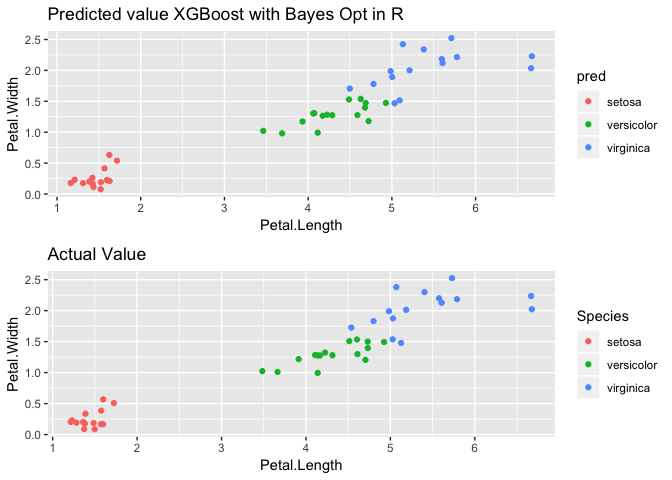
\includegraphics{PythonInR_files/figure-latex/xgb.Bayesopt-1.pdf}

\begin{Shaded}
\begin{Highlighting}[]
\ImportTok{import}\NormalTok{ math}
\ImportTok{import}\NormalTok{ os}
\NormalTok{os.environ[}\StringTok{'KMP_DUPLICATE_LIB_OK'}\NormalTok{]}\OperatorTok{=}\StringTok{'True'}
\ImportTok{from}\NormalTok{ bayes_opt }\ImportTok{import}\NormalTok{ BayesianOptimization}
\ImportTok{import}\NormalTok{ xgboost }\ImportTok{as}\NormalTok{ xgb}
\ImportTok{from}\NormalTok{ xgboost }\ImportTok{import}\NormalTok{ XGBClassifier}

\CommentTok{#Let's use the same dataset above}
\NormalTok{df_iris2.head(}\DecValTok{5}\NormalTok{)}
\end{Highlighting}
\end{Shaded}

\begin{verbatim}
##    SepalLength  SepalWidth  PetalLength  PetalWidth  Species
## 0          5.1         3.5          1.4         0.2      0.0
## 1          4.9         3.0          1.4         0.2      0.0
## 2          4.7         3.2          1.3         0.2      0.0
## 3          4.6         3.1          1.5         0.2      0.0
## 4          5.0         3.6          1.4         0.2      0.0
\end{verbatim}

\begin{Shaded}
\begin{Highlighting}[]
\NormalTok{df_iris2.shape}
\end{Highlighting}
\end{Shaded}

\begin{verbatim}
## (150, 5)
\end{verbatim}

\begin{Shaded}
\begin{Highlighting}[]
\NormalTok{Y }\OperatorTok{=}\NormalTok{ df_iris2.Species}
\NormalTok{X }\OperatorTok{=}\NormalTok{ df_iris2.iloc[:,}\DecValTok{0}\NormalTok{:}\DecValTok{4}\NormalTok{]}

\NormalTok{X_train, X_test, y_train, y_test }\OperatorTok{=}\NormalTok{ train_test_split(X, Y, test_size}\OperatorTok{=}\FloatTok{0.3}\NormalTok{, random_state}\OperatorTok{=}\DecValTok{42}\NormalTok{)}

\NormalTok{XGB_dtrain }\OperatorTok{=}\NormalTok{ xgb.DMatrix(X_train, label}\OperatorTok{=}\NormalTok{y_train)}
\end{Highlighting}
\end{Shaded}

\begin{verbatim}
## /anaconda3/lib/python3.7/site-packages/xgboost/core.py:587: FutureWarning: Series.base is deprecated and will be removed in a future version
##   if getattr(data, 'base', None) is not None and \
\end{verbatim}

\begin{Shaded}
\begin{Highlighting}[]
\NormalTok{XGB_dtest }\OperatorTok{=}\NormalTok{ xgb.DMatrix(X_test)}

\KeywordTok{def}\NormalTok{ xgb_evaluate(max_depth,subsample,colsample_bytree,min_child_weight,reg_lambda,reg_alpha,gamma):}
\NormalTok{    params}\OperatorTok{=}\NormalTok{\{}\StringTok{'eval_metric'}\NormalTok{:}\StringTok{'mlogloss'}\NormalTok{,}
            \StringTok{'objective'}\NormalTok{:}\StringTok{'multi:softprob'}\NormalTok{,}
            \StringTok{'num_class'}\NormalTok{:}\DecValTok{3}\NormalTok{,}
            \StringTok{'booster'}\NormalTok{:}\StringTok{'gbtree'}\NormalTok{,}
           \StringTok{'max_depth'}\NormalTok{:}\BuiltInTok{int}\NormalTok{(max_depth),}
            \StringTok{'subsample'}\NormalTok{:subsample,}
            \StringTok{'colsample_bytree'}\NormalTok{:colsample_bytree,}
            \StringTok{'min_child_weight'}\NormalTok{:}\BuiltInTok{int}\NormalTok{(min_child_weight),}
            \StringTok{'reg_lambda'}\NormalTok{:reg_lambda,}
            \StringTok{'reg_alpha'}\NormalTok{: reg_alpha,}
            \StringTok{'gamma'}\NormalTok{:gamma,}
           \StringTok{'eta'}\NormalTok{:}\FloatTok{0.008}\NormalTok{\}}
\NormalTok{    cv }\OperatorTok{=}\NormalTok{ xgb.cv(params, XGB_dtrain, num_boost_round}\OperatorTok{=}\DecValTok{10}\NormalTok{,nfold}\OperatorTok{=}\DecValTok{3}\NormalTok{)}
    \ControlFlowTok{return}\NormalTok{ cv[}\StringTok{'test-mlogloss-mean'}\NormalTok{].iloc[}\OperatorTok{-}\DecValTok{1}\NormalTok{]}

\NormalTok{xgb_bo }\OperatorTok{=}\NormalTok{ BayesianOptimization(xgb_evaluate,}
\NormalTok{                             \{}\StringTok{'max_depth'}\NormalTok{:(}\DecValTok{1}\NormalTok{,}\DecValTok{5}\NormalTok{),}
                             \StringTok{'subsample'}\NormalTok{:(}\FloatTok{0.6}\NormalTok{,}\DecValTok{1}\NormalTok{),}
                             \StringTok{'colsample_bytree'}\NormalTok{:(}\FloatTok{0.6}\NormalTok{,}\DecValTok{1}\NormalTok{),}
                             \StringTok{'min_child_weight'}\NormalTok{:(}\DecValTok{1}\NormalTok{,}\DecValTok{10}\NormalTok{),}
                             \StringTok{'reg_lambda'}\NormalTok{:(}\FloatTok{0.001}\NormalTok{,}\DecValTok{1}\NormalTok{),}
                             \StringTok{'reg_alpha'}\NormalTok{:(}\FloatTok{0.001}\NormalTok{,}\DecValTok{1}\NormalTok{),}
                             \StringTok{'gamma'}\NormalTok{:(}\FloatTok{0.1}\NormalTok{,}\DecValTok{2}\NormalTok{)\})}

\NormalTok{xgb_bo.maximize(init_points}\OperatorTok{=}\DecValTok{3}\NormalTok{,n_iter}\OperatorTok{=}\DecValTok{5}\NormalTok{,acq}\OperatorTok{=}\StringTok{'ei'}\NormalTok{)}
\end{Highlighting}
\end{Shaded}

\begin{verbatim}
## |   iter    |  target   | colsam... |   gamma   | max_depth | min_ch... | reg_alpha | reg_la... | subsample |
## -------------------------------------------------------------------------------------------------------------
## |  1        |  1.047    |  0.6232   |  1.394    |  2.668    |  9.625    |  0.4137   |  0.3722   |  0.8337   |
## |  2        |  1.021    |  0.9954   |  0.7141   |  3.812    |  2.452    |  0.3431   |  0.8103   |  0.826    |
## |  3        |  1.026    |  0.6968   |  1.989    |  4.328    |  8.731    |  0.5102   |  0.6545   |  0.9698   |
## |  4        |  1.093    |  0.6      |  0.1      |  1.0      |  10.0     |  0.001    |  0.001    |  0.6      |
## |  5        |  1.092    |  1.0      |  0.1      |  5.0      |  10.0     |  0.001    |  0.001    |  0.6      |
## |  6        |  1.068    |  0.8847   |  0.1631   |  2.206    |  9.981    |  0.09808  |  0.9286   |  0.6482   |
## |  7        |  1.049    |  0.6118   |  0.1002   |  3.961    |  9.786    |  0.9661   |  0.02062  |  0.8252   |
## |  8        |  1.051    |  0.9755   |  0.174    |  1.067    |  9.671    |  0.09348  |  0.07553  |  0.7078   |
## =============================================================================================================
\end{verbatim}

\begin{Shaded}
\begin{Highlighting}[]
\NormalTok{xgb_bo.}\BuiltInTok{max}
\end{Highlighting}
\end{Shaded}

\begin{verbatim}
## {'target': 1.0926586666666667, 'params': {'colsample_bytree': 0.6, 'gamma': 0.1, 'max_depth': 1.0, 'min_child_weight': 10.0, 'reg_alpha': 0.001, 'reg_lambda': 0.001, 'subsample': 0.6}}
\end{verbatim}

\begin{Shaded}
\begin{Highlighting}[]
\NormalTok{bo_params}\OperatorTok{=}\NormalTok{xgb_bo.}\BuiltInTok{max}\NormalTok{[}\StringTok{'params'}\NormalTok{]}

\NormalTok{bo_params[}\StringTok{'max_depth'}\NormalTok{] }\OperatorTok{=} \BuiltInTok{int}\NormalTok{(}\BuiltInTok{round}\NormalTok{(bo_params[}\StringTok{'max_depth'}\NormalTok{]))}
\NormalTok{bo_params[}\StringTok{'min_child_weight'}\NormalTok{] }\OperatorTok{=} \BuiltInTok{int}\NormalTok{(}\BuiltInTok{round}\NormalTok{(bo_params[}\StringTok{'min_child_weight'}\NormalTok{]))}

\NormalTok{bo_params}
\end{Highlighting}
\end{Shaded}

\begin{verbatim}
## {'colsample_bytree': 0.6, 'gamma': 0.1, 'max_depth': 1, 'min_child_weight': 10, 'reg_alpha': 0.001, 'reg_lambda': 0.001, 'subsample': 0.6}
\end{verbatim}

\begin{Shaded}
\begin{Highlighting}[]
\NormalTok{XGB_fit }\OperatorTok{=}\NormalTok{ xgb.train(bo_params,XGB_dtrain,num_boost_round }\OperatorTok{=} \DecValTok{100}\NormalTok{)}
\NormalTok{pred }\OperatorTok{=}\NormalTok{ XGB_fit.predict(XGB_dtest)}

\NormalTok{pred }\OperatorTok{=}\NormalTok{ pred.}\BuiltInTok{round}\NormalTok{()}
\NormalTok{pred }\OperatorTok{+=} \FloatTok{0.}
\NormalTok{pd.crosstab(pred, y_test, rownames }\OperatorTok{=}\NormalTok{ [}\StringTok{'pred'}\NormalTok{], colnames}\OperatorTok{=}\NormalTok{[}\StringTok{'actual'}\NormalTok{])}
\CommentTok{#100%}
\end{Highlighting}
\end{Shaded}

\begin{verbatim}
## actual  0.0  1.0  2.0
## pred                 
## 0.0      19    0    0
## 1.0       0   13    0
## 2.0       0    0   13
\end{verbatim}

\begin{Shaded}
\begin{Highlighting}[]
\NormalTok{plt.subplot(}\DecValTok{1}\NormalTok{, }\DecValTok{2}\NormalTok{, }\DecValTok{1}\NormalTok{)}
\NormalTok{plt.scatter(X_test.PetalLength, X_test.PetalWidth, c}\OperatorTok{=}\NormalTok{pred)}
\NormalTok{plt.title(}\StringTok{'Predicted value by XGboost with Bayes Opt in Python'}\NormalTok{)}
\NormalTok{plt.subplot(}\DecValTok{1}\NormalTok{, }\DecValTok{2}\NormalTok{, }\DecValTok{2}\NormalTok{)}
\NormalTok{plt.scatter(X_test.PetalLength, X_test.PetalWidth, c}\OperatorTok{=}\NormalTok{y_test)}
\NormalTok{plt.title(}\StringTok{'Actual value'}\NormalTok{)}
\NormalTok{plt.show()}
\end{Highlighting}
\end{Shaded}

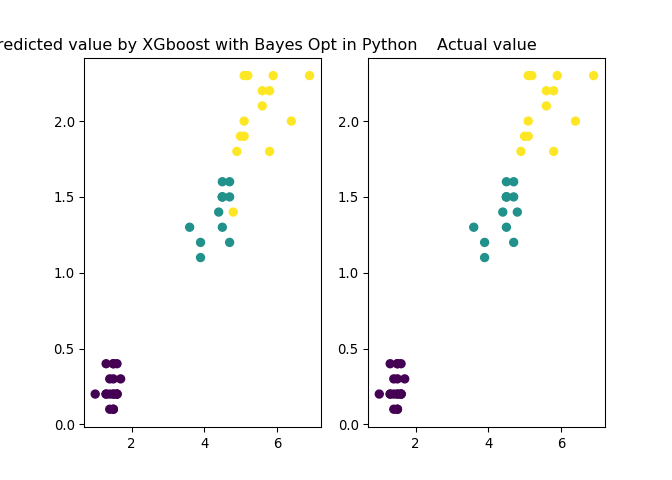
\includegraphics{PythonInR_files/figure-latex/BayesOpt-1.pdf}


\end{document}
